\documentclass[9pt,handout]{beamer}
% beamerthemeFeng.sty
% style file for beamer presentation

% tikz is used to ``draw'' title page and other templates in beamer
\usepackage{tikz,etoolbox}
\usetikzlibrary{shapes,arrows}

\definecolor{UWBlack}{HTML}{000000}
\definecolor{UWWhite}{HTML}{FFFFFF}


\definecolor{UWMathPinkL1}{HTML}{FFBEEF}
\definecolor{UWMathPinkL2}{HTML}{FF63AA}
\definecolor{UWMathPinkL3}{HTML}{DF2498}
\definecolor{UWMathPinkL4}{HTML}{C60078}
\definecolor{UWGrayL1}{HTML}{DFDFDF}
\definecolor{UWGrayL2}{HTML}{A2A2A2}
\definecolor{UWGrayL3}{HTML}{787878}
\definecolor{UWGrayL4}{HTML}{000000}
\definecolor{UWGoldL1}{HTML}{FFFFAA}
\definecolor{UWGoldL2}{HTML}{FFEA3D}
\definecolor{UWGoldL3}{HTML}{FFD54F}
\definecolor{UWGoldL4}{HTML}{E4B429}

\definecolor{carrot}{HTML}{EE693F}
\definecolor{ivory}{HTML}{F1F3CE}
\definecolor{emerald}{HTML}{265C00}
\definecolor{turquise}{HTML}{5BC8AC}
\definecolor{peacockblue}{HTML}{1E656D}
\definecolor{spicy}{HTML}{B51D0A}
\definecolor{bluegreen}{HTML}{5F968E}
\definecolor{rust}{HTML}{9B4F0F}
\definecolor{burntorange}{HTML}{DE7A22}
\definecolor{sea}{HTML}{20948B}
\definecolor{lagoon}{HTML}{6AB187}


% Set colors for different components in a slide
\setbeamercolor{background canvas}{bg=UWWhite}
\setbeamercolor{author}{fg=UWGoldL3}
\setbeamercolor{institute}{fg=UWMathPinkL3}
\setbeamercolor{title}{fg=UWGrayL4}
\setbeamercolor{section in head/foot}{bg=UWBlack, fg=UWGoldL3}
\setbeamercolor{author in head/foot}{fg=UWGoldL3, bg=UWBlack}
\setbeamercolor{title in head/foot}{fg=UWBlack,bg=UWGoldL3}
\setbeamercolor{institute in head/foot}{fg=UWGoldL3, bg=UWBlack}
\setbeamercolor{navigation symbols}{fg=UWBlack}
\setbeamercolor{normal text}{fg=UWGrayL3}
\setbeamercolor{section in toc}{fg=emerald}
\setbeamercolor{subsection in toc}{fg=bluegreen}
\setbeamercolor{frametitle}{fg=UWMathPinkL2, bg=UWGrayL1}
\setbeamercolor{block title}{bg=emerald, fg=ivory}
\setbeamercolor{block body}{bg=peacockblue!20, fg=peacockblue}
\setbeamercolor{section number projected}{bg=turquise,fg=black}
\setbeamercolor{block title example}{fg=rust,
	bg= sea!40}
\setbeamercolor{block body example}{fg= burntorange,
	bg= lagoon!20}

\setbeamerfont{frametitle}{series=\bfseries} % bold frame title
\setbeamerfont{section number projected}{% bold TOC bullet
  family=\rmfamily,series=\bfseries,size=\normalsize}
  
% two common fields in conference presentations
\newcommand\jointwork[1]{\def\insertjointwork{#1}}
\newcommand\conference[1]{\def\insertconference{#1}}

% Title page style
\setbeamertemplate{title page}{
\begin{tikzpicture}[remember picture, overlay]
\fill[UWWhite]
  ([yshift=30pt]current page.west) rectangle (current page.south east);

\fill[UWBlack]
  ([yshift=30pt]current page.west) rectangle (current page.north east);

\node[anchor=east] at ([yshift=-50pt,xshift=-15pt]current page.north east)
  {
  
\includegraphics[width=0.4\linewidth]{./UniversityOfWaterloo_logo_vert_rev_rgb.png}};

\node[anchor=north west] at ([yshift=-70pt,xshift=15pt]current page.north west) (institute)
	{
	\parbox[t]{.78\paperwidth}{
    \usebeamerfont{institute}\usebeamercolor[fg]{institute}\large\bfseries\insertinstitute}
    };
    
\node[anchor=west] at ([yshift=-45pt,xshift=15pt]current page.north west) (author)
	{
	\parbox[t]{.78\paperwidth}{
    \usebeamerfont{author}\usebeamercolor[fg]{author}\Large\bfseries \insertauthor}
    };


    
\node[anchor=north] at ([yshift=15pt]current page.center) (title)
	{
	\parbox[t]{\textwidth}{\huge\bfseries\centering
	\usebeamerfont{title}\usebeamercolor[fg]{title}\inserttitle}
	};
    
\node[anchor=north] at ([yshift=-40pt]current page.center) (jointwork)
	{
	\parbox[t]{\paperwidth}{\bfseries\centering\insertjointwork}
	};
	
\node[anchor=north] at ([yshift=40pt]current page.south) (jointwork)
	{
	\parbox[t]{\paperwidth}{\centering\insertconference}
	};
\end{tikzpicture}
}

\setbeamertemplate{headline} % add navigation to headline
{%
  \begin{beamercolorbox}{section in head/foot}
    \vskip5pt\bfseries
    \insertnavigation{\paperwidth}
    \vskip2pt
  \end{beamercolorbox}%
}


\renewcommand*{\slideentry}[6]{} % no solid circle in headline

% three-parts footline, color determined in beamer template
\setbeamertemplate{footline}
{
	\leavevmode % vertical mode is ended and horizontal mode is entered. In vertical mode, TeX stacks horizontal boxes vertically, whereas in horizontal mode, they are taken as part of the text line. 
	\begin{beamercolorbox}[wd=.333333\paperwidth,ht=2.5ex,dp=1.125ex,
      leftskip=.3cm,rightskip=.3cm plus1fil]{author in head/foot}
		\usebeamerfont{author in head/foot}\insertshortauthor
    \end{beamercolorbox}%
    \begin{beamercolorbox}[wd=.333333\paperwidth,ht=2.5ex,dp=1.125ex,
      leftskip=.3cm,rightskip=.3cm plus1fil,center]{title in head/foot}
      {\usebeamerfont{title in head/foot}\insertshorttitle}
    \end{beamercolorbox}%
    \begin{beamercolorbox}[wd=.333333\paperwidth,ht=2.5ex,dp=1.125ex,
      leftskip=.3cm,rightskip=.3cm plus1fil]{institute in head/foot}
      \hfill    {\usebeamercolor[fg]{institute in head/foot}\insertshortinstitute}    
	\end{beamercolorbox}%
}

\setbeamertemplate{navigation symbols}{\bfseries\insertframenumber/\inserttotalframenumber}

\setbeamertemplate{sections/subsections in toc}[ball]

% make the itemize bullets pixelated >
\setbeamertemplate{itemize item}{
	\tikz{
		\draw[fill=spicy,draw=none] (0, 0) rectangle(0.075, 0.075);
		\draw[fill=spicy,draw=none] (0.075, 0.075) rectangle(0.15, 0.15);
		\draw[fill=spicy,draw=none] (0, 0.15) rectangle(0.075, 0.225);
	}
}

% make the subitems also pixelated >, but a little smaller and red
\setbeamertemplate{itemize subitem}{
	\tikz{
		\draw[fill=carrot,draw=none] (0, 0) rectangle(0.05, 0.05);
		\draw[fill=carrot,draw=none] (0.05, 0.05) rectangle(0.1, 0.1);
		\draw[fill=carrot,draw=none] (0, 0.1) rectangle(0.05, 0.15);
	}
}

\AtBeginEnvironment{block}{
	\setbeamertemplate{itemize item}{
		\tikz{
			\draw[fill=spicy,draw=none] (0, 0) rectangle(0.075, 0.075);
			\draw[fill=spicy,draw=none] (0.075, 0.075) rectangle(0.15, 0.15);
			\draw[fill=spicy,draw=none] (0, 0.15) rectangle(0.075, 0.225);
		}
	}

	\setbeamertemplate{itemize subitem}{
		\tikz{
			\draw[fill=carrot,draw=none] (0, 0) rectangle(0.05, 0.05);
			\draw[fill=carrot,draw=none] (0.05, 0.05) rectangle(0.1, 0.1);
			\draw[fill=carrot,draw=none] (0, 0.1) rectangle(0.05, 0.15);
		}
	}
}

\setbeamertemplate{blocks}[rounded][shadow=false]

\setbeamercovered{invisible}

\usefonttheme[onlymath]{serif} % change the math font theme

\AtBeginEnvironment{theorem}{%
  \setbeamercolor{block title}{bg=peppercorn, fg=pearl}
  \setbeamercolor{block body}{bg=parsnip, fg=spicy}
}

% set color scheme in different parts 
% please refer to beamer cheatsheet below for details
% http://www.cpt.univ-mrs.fr/~masson/latex/Beamer-appearance-cheat-sheet.pdf

\usepackage{amsmath, amsthm,amsfonts, amssymb, amscd}
\newtheorem{postulate}{Postulate}
\newtheorem{remark}{Remark}
\allowdisplaybreaks
\usepackage{appendixnumberbeamer}
%\usepackage[backend=bibtex,citestyle=authoryear-icomp,natbib,maxcitenames=1]{biblatex}
%\addbibresource{bibfile.bib}
\usepackage{cancel}
\usepackage{float}
\usepackage{graphicx}
\graphicspath{ {./images/} }
\usepackage{hyperref}
\usepackage{mathtools}

\title[\textbf{Bundles in Classical Gauge Field Theory}]{Bundles in Classical Gauge Field Theory}

\author[\textbf{Sid (s3bhatta@uwaterloo.ca)}]
{Siddhartha Bhattacharjee \\
s3bhatta@uwaterloo.ca \\
Discord: booodaness}

\institute[\textbf{University of Waterloo, Mathematical Physics}]
{Mathematical Physics (1C) \\
University of Waterloo
}

\jointwork{}
\conference{Canadian Undergraduate Mathematics Conference, University of Toronto, 2023}

\begin{document}

{
\beamertemplatenavigationsymbolsempty
\begin{frame}[plain]
\titlepage
\end{frame}
}

{
\beamertemplatenavigationsymbolsempty
\defbeamertemplate*{headline}{miniframes theme no subsection no content}
{\begin{beamercolorbox}{section in head/foot}
\vskip\headheight
\end{beamercolorbox}}

\begin{frame}{Outline} 
\tableofcontents 
\end{frame} 
}
\addtocounter{framenumber}{-2}

\section{Classical Gauge Fields}

\subsection{Classical Fields}

\subsubsection{Definition}
\begin{frame}{Definition}
\begin{itemize}
\item Let $\mathcal{M}$ be a pseudo-Riemannian manifold with a metric $g$. A classical field $\phi$ of rank $\left( p, q \right)$ is a differentiable tensor field living on $\mathcal{M}$ i.e.,

\begin{block}{As a differentiable tensor field}
\begin{itemize}
\item $\displaystyle{\phi : \mathcal{M} \to \left( \prod_{i=1}^{p} V^* \times \prod_{j=1}^q V \to \mathbb{R} \right)}$
\item $\phi \in C \left( \mathcal{M} \right)$
\end{itemize}
\end{block}

where $V$ is a vector space with $\mathbb{R}$ as the base field.

\item This is the starting point for defining classical fields. Additionally, they obey some physical properties discussed below.

\begin{block}{Physical properties}
\begin{enumerate}
\item Stationary-action principle
\item Local Lorentz invariance
\item Gauge invariance
\end{enumerate}
\end{block}

\end{itemize}
\end{frame}

\subsubsection{Stationary-action Principle}
\begin{frame}{Stationary-action Principle}
\begin{itemize}
\item Let the function space of $\phi$, i.e. $\displaystyle{\left[ \mathcal{M} \to \left( \prod_{i=1}^{p} V^* \times \prod_{j=1}^q V \to \mathbb{R} \right) \right] \cap C \left( \mathcal{M} \right)}$, be denoted as $\mathcal{F}$.

\begin{definition}[Lagrangian]
The Lagrangian [density] $\mathcal{L}$ of a classical field $\phi$ is a differentiable map $\mathcal{L} : \mathcal{F} \times T^* \mathcal{M} \times \mathcal{M} \to \mathbb{R}$.
\end{definition}

Here, $T^* \mathcal{M}$ denotes the cotangent bundle of $\mathcal{M}$.

\item However, we have not yet motivated bundles. Therefore, for now, we will think of $T^* \mathcal{M}$ as being set-theoretically isomorphic to the set of covariant derivatives of $\phi$ along every continuous curve $\gamma$ in $\mathcal{M}$,

$$T^* \mathcal{M} \cong_{\text{set}} \left\{ \nabla_\gamma \phi \: \vert \: \gamma : \left[ 0, 1 \right] \to \mathcal{M} \text{ is continuous} \right\}$$

\item By continuous curves, we refer to the topological notion of the continuity of maps from the topological space $\left( \left[ 0, 1 \right], \mathcal{O}_{\mathbb{R}} \big\vert_{\left[ 0, 1 \right]} \right)$ to $\left( \mathcal{M}, \mathcal{O}_{\mathcal{M}} \right)$.

Here, $\mathcal{O}_{\mathbb{R}} \big\vert_{\left[ 0, 1 \right]}$ is the subspace topology induced on the unit interval by the Euclidean topology on $\mathbb{R}$ and $\mathcal{O}_{\mathcal{M}}$ is the manifold topology on $\mathcal{M}$.

\end{itemize}
\end{frame}

\begin{frame}{}
\begin{definition}[Action]
The action for a tensor field $\phi$ in a compact neighbourhood $U \subset \mathcal{M}$ is the linear functional,

$$S \left[ \phi \right] : = \int_{x \in U} \varepsilon \mathcal{L} \left( \phi \left( x \right), T^*_{x} \mathcal{M}, x \right)$$

where $\varepsilon$ is the Riemannian volume form which in local coordinates can be written as,

$$\varepsilon : = \sqrt{\left\lvert \det \left( g \right) \right\rvert} \bigwedge_{\mu} \text{d}x^\mu$$
\end{definition}

In local coordinates, using index notation, the action can be covariantly written in terms of components as,

$$S \left[ \phi \left( x^\alpha \right) \right] = \int_{U} \varepsilon \mathcal{L} \left( \phi^{\rho_1 \dots \rho_p}_{\phantom{\rho_1 \dots \rho_p} \lambda_1 \dots \lambda_q}, \nabla_\mu \phi^{\rho_1 \dots \rho_p}_{\phantom{\rho_1 \dots \rho_p} \lambda_1 \dots \lambda_q}, x^\alpha \right)$$

where $\phi^{\rho_1 \dots \rho_p}_{\phantom{\rho_1 \dots \rho_p} \lambda_1 \dots \lambda_q} = \underset{i=1}{\overset{p}{\bigcirc}} \text{d}x^{\rho_i} \circ \underset{j=1}{\overset{q}{\bigcirc}} \partial_{\lambda_j} \left( \phi \right)$.
\end{frame}

\begin{frame}
\begin{postulate}[Stationary-principle action]
For on-shell trajectories $\phi \in \mathcal{F}$, we have the following for all compact neighbourhoods $U \subset \mathcal{M}$,

$$\delta S \left[ \phi \right] = 0$$
\end{postulate}

i.e.,

$$\delta \int_{U} \varepsilon \mathcal{L} \left( \phi^{\rho_1 \dots \rho_p}_{\phantom{\rho_1 \dots \rho_p} \lambda_1 \dots \lambda_q}, \nabla_\mu \phi^{\rho_1 \dots \rho_p}_{\phantom{\rho_1 \dots \rho_p} \lambda_1 \dots \lambda_q}, x^\alpha \right) = 0$$


\begin{block}{Theorem (Euler-Lagrange equations)}
A classical field $\phi$ is on-shell i.e. obeys the principle of stationary action if and only if it satisfies the Euler-Lagrange equations:

$$\frac{\partial \mathcal{L}}{\partial \phi^{\rho_1 \dots \rho_p}_{\phantom{\rho_1 \dots \rho_p} \lambda_1 \dots \lambda_q}} - \nabla_\mu \frac{\partial \mathcal{L}}{\partial \left( \nabla_\mu \phi^{\rho_1 \dots \rho_p}_{\phantom{\rho_1 \dots \rho_p} \lambda_1 \dots \lambda_q} \right)} = 0$$

with summation over dummy indices implied (Einstein summation convention).
\end{block}
\end{frame}

\begin{frame}{}
\begin{block}{Proof.}
\begin{align*}
\delta S & = 0 \\ 
\delta \int_{U} \varepsilon \mathcal{L} & = 0 \\ 
\hline \\
\int_{U} \varepsilon \left[ \delta \phi^{\rho_1 \dots \rho_p}_{\phantom{\rho_1 \dots \rho_p} \lambda_1 \dots \lambda_q} \frac{\partial \mathcal{L}}{\partial \phi^{\rho_1 \dots \rho_p}_{\phantom{\rho_1 \dots \rho_p} \lambda_1 \dots \lambda_q}} \right. \\ 
+ \left. \delta \left( \nabla_\mu \phi^{\rho_1 \dots \rho_p}_{\phantom{\rho_1 \dots \rho_p} \lambda_1 \dots \lambda_q} \right) \frac{\partial \mathcal{L}}{\partial \left( \nabla_\mu \phi^{\rho_1 \dots \rho_p}_{\phantom{\rho_1 \dots \rho_p} \lambda_1 \dots \lambda_q} \right)} \right] & = 0 \\ 
\hline \\
\int_{U} \varepsilon \left[ \delta \phi^{\rho_1 \dots \rho_p}_{\phantom{\rho_1 \dots \rho_p} \lambda_1 \dots \lambda_q} \frac{\partial \mathcal{L}}{\partial \phi^{\rho_1 \dots \rho_p}_{\phantom{\rho_1 \dots \rho_p} \lambda_1 \dots \lambda_q}} \right. \\ 
+ \left. \nabla_\mu \left( \delta \phi^{\rho_1 \dots \rho_p}_{\phantom{\rho_1 \dots \rho_p} \lambda_1 \dots \lambda_q} \right) \frac{\partial \mathcal{L}}{\partial \left( \nabla_\mu \phi^{\rho_1 \dots \rho_p}_{\phantom{\rho_1 \dots \rho_p} \lambda_1 \dots \lambda_q} \right)} \right] & = 0
\end{align*}
\end{block}
\end{frame}

\begin{frame}{}
\begin{block}{Proof (continued).}
\begin{align*}
\int_{U} \varepsilon \delta \phi^{\rho_1 \dots \rho_p}_{\phantom{\rho_1 \dots \rho_p} \lambda_1 \dots \lambda_q} \frac{\partial \mathcal{L}}{\partial \phi^{\rho_1 \dots \rho_p}_{\phantom{\rho_1 \dots \rho_p} \lambda_1 \dots \lambda_q}} \\ 
+ \frac{\partial \mathcal{L}}{\partial \left( \nabla_\mu \phi^{\rho_1 \dots \rho_p}_{\phantom{\rho_1 \dots \rho_p} \lambda_1 \dots \lambda_q} \right)} \cancel{\int_{U} \varepsilon \nabla_\mu \left( \delta \phi^{\rho_1 \dots \rho_p}_{\phantom{\rho_1 \dots \rho_p} \lambda_1 \dots \lambda_q} \right)} \\
- \int_{U} \varepsilon \left[ \nabla_\mu \frac{\partial \mathcal{L}}{\partial \left( \nabla_\mu \phi^{\rho_1 \dots \rho_p}_{\phantom{\rho_1 \dots \rho_p} \lambda_1 \dots \lambda_q} \right)} \int \varepsilon \nabla_\mu \left( \delta \phi^{\rho_1 \dots \rho_p}_{\phantom{\rho_1 \dots \rho_p} \lambda_1 \dots \lambda_q} \right) \right] & = 0 \\
\hline \\
\int_{U} \varepsilon \delta \phi^{\rho_1 \dots \rho_p}_{\phantom{\rho_1 \dots \rho_p} \lambda_1 \dots \lambda_q} \frac{\partial \mathcal{L}}{\partial \phi^{\rho_1 \dots \rho_p}_{\phantom{\rho_1 \dots \rho_p} \lambda_1 \dots \lambda_q}} \\ 
- \int_{U} \varepsilon \left[ \delta \phi^{\rho_1 \dots \rho_p}_{\phantom{\rho_1 \dots \rho_p} \lambda_1 \dots \lambda_q} \nabla_\mu \frac{\partial \mathcal{L}}{\partial \left( \nabla_\mu \phi^{\rho_1 \dots \rho_p}_{\phantom{\rho_1 \dots \rho_p} \lambda_1 \dots \lambda_q} \right)} \right] & = 0 \\
\end{align*}
\end{block}	
\end{frame}

\begin{frame}{}
\begin{block}{Proof (continued).}
$$\int_{U} \varepsilon \delta \phi^{\rho_1 \dots \rho_p}_{\phantom{\rho_1 \dots \rho_p} \lambda_1 \dots \lambda_q} \left[ \frac{\partial \mathcal{L}}{\partial \phi^{\rho_1 \dots \rho_p}_{\phantom{\rho_1 \dots \rho_p} \lambda_1 \dots \lambda_q}} - \nabla_\mu \frac{\partial \mathcal{L}}{\partial \left( \nabla_\mu \phi^{\rho_1 \dots \rho_p}_{\phantom{\rho_1 \dots \rho_p} \lambda_1 \dots \lambda_q} \right)} \right] = 0$$

Since the above is true for all compact neighbourhoods $U \subset \mathcal{M}$, by the fundamental lemma of the calculus of variations,

$$\frac{\partial \mathcal{L}}{\partial \phi^{\rho_1 \dots \rho_p}_{\phantom{\rho_1 \dots \rho_p} \lambda_1 \dots \lambda_q}} - \nabla_\mu \frac{\partial \mathcal{L}}{\partial \left( \nabla_\mu \phi^{\rho_1 \dots \rho_p}_{\phantom{\rho_1 \dots \rho_p} \lambda_1 \dots \lambda_q} \right)} = 0 \qed$$
\end{block}

The power of the above functional-analytic manipulations and notions is that the above statements are all logically equivalent, therefore proving 'S-A principle iff E-L equations'. 
\end{frame}

\subsubsection{Local Lorentz Invariance}
\begin{frame}{Local Lorentz Invariance}
\begin{itemize}
\item Local Lorentz invariance is the idea that at each $p \in \mathcal{M}$, the action of the restricted Lorentz group $\text{SO}^+ \left( 1, 3 \right)$ on tensorial objects living on $T_p \mathcal{M}$, leaves them invariant.

\item This means that the components of a rank $\left( p, q \right)$ tensor field $T$ with components $T^{\rho_1 \dots \rho_p}_{\phantom{\rho_1 \dots \rho_p} \lambda_1 \dots \lambda_q}$ must transform covariantly with respect to the restricted Lorentz group. 

In other words, we require that for any pair of primed and unprimed coordinate systems related by some transformation $\Lambda \in \text{SO}^+ \left( 1, 3 \right)$, the following principle applies:

\begin{postulate}[Local Lorentz invariance]
$$T = T^\prime$$
\end{postulate}

This simple principle has far-reaching consequences in theoretical physics, such as severe restriction induced on the form of physical laws and equations.
\end{itemize}	
\end{frame}

\begin{frame}
\begin{block}{Theorem (Tensor component transformation law)}
Invariance holds if and only if for a tensor field $T$, its components transform under any $\Lambda \in \text{SO}^+ \left( 1, 3 \right)$ represented by (in terms of its action on the concerned tangent space) a Jacobian with components $\displaystyle{\Lambda^{\mu^\prime}_{\phantom{\mu^\prime} \mu} = \frac{\partial x^{\mu^\prime}}{\partial x^\mu}}$ as,

$$T^{\rho_{1^\prime} \dots \rho_{p^\prime}}_{\phantom{\rho_{1^\prime} \dots \rho_{p^\prime}} \lambda_{1^\prime} \dots \lambda_{q^\prime}} = \left( \prod_{i=1}^{p} \Lambda^{\rho_i^\prime}_{\phantom{\rho_i^\prime} \rho_i} \right) T^{\rho_1 \dots \rho_p}_{\phantom{\rho_1 \dots \rho_p} \lambda_1 \dots \lambda_q} \left( \prod_{j=1}^{q} \dots \Lambda^{\lambda_j}_{\phantom{\lambda_j} \lambda_j^\prime} \right)$$
\end{block}

\begin{block}{Proof.}
By local Lorentz invariance,

\begin{align*}
T^{\rho_{1^\prime} \dots \rho_{p^\prime}}_{\phantom{\rho_{1^\prime} \dots \rho_{p^\prime}} \lambda_{1^\prime} \dots \lambda_{q^\prime}} & : = T \left( \text{d}x^{\rho_{1^\prime}}, \dots, \text{d}x^{\rho_{p^\prime}}, \partial_{\lambda_{1^\prime}}, \dots, \partial_{\lambda_{q^\prime}} \right) \\
& = T \left( \frac{\partial x^{\rho_{1^\prime}}}{\partial x^{\rho_1}} \text{d}x^{\rho_1}, \dots, \frac{\partial x^{\rho_{p^\prime}}}{\partial x^{\rho_p}} \text{d}x^{\rho_p}, \frac{\partial x^{\lambda_1}}{\partial \lambda_{1^\prime}} \partial_{\lambda_1}, \dots, \frac{\partial x^{\lambda_q}}{\partial \lambda_{q^\prime}} \partial_{\lambda_q} \right)
\end{align*}
\end{block}
\end{frame}

\begin{frame}
\begin{block}{Proof (continued).}
Since a tensor is a multilinear map,
	
\begin{align*}
T^{\rho_{1^\prime} \dots \rho_{p^\prime}}_{\phantom{\rho_{1^\prime} \dots \rho_{p^\prime}} \lambda_{1^\prime} \dots \lambda_{q^\prime}} & = \left( \prod_{i=1}^{p} \frac{\partial x^{\rho_{i^\prime}}}{\partial x^{\rho_i}} \right) T \left( \text{d}x^{\rho_1}, \dots, \text{d}x^{\rho_p}, \partial_{\lambda_1}, \dots, \partial_{\lambda_q} \right) \left( \prod_{j=1}^{q} \frac{\partial x^{\lambda_j}}{\partial \lambda_{j^\prime}} \right) \\
& = \left( \prod_{i=1}^{p} \frac{\partial x^{\rho_{i^\prime}}}{\partial x^{\rho_i}} \right) T^{\rho_1 \dots \rho_p}_{\phantom{\rho_1 \dots \rho_p} \lambda_1 \dots \lambda_q} \left( \prod_{j=1}^{q} \frac{\partial x^{\lambda_j}}{\partial \lambda_{j^\prime}} \right) \\
& = \left( \prod_{i=1}^{p} \Lambda^{\rho_i^\prime}_{\phantom{\rho_i^\prime} \rho_i} \right) T^{\rho_1 \dots \rho_p}_{\phantom{\rho_1 \dots \rho_p} \lambda_1 \dots \lambda_q} \left( \prod_{j=1}^{q} \dots \Lambda^{\lambda_j}_{\phantom{\lambda_j} \lambda_j^\prime} \right) \qquad \quad \qed
\end{align*}
\end{block}
\end{frame}

\subsubsection{Gauge Invariance}
\begin{frame}{Gauge Invariance}
\begin{block}{Observational equivalence}
In classical field theory, observational equivalence is the idea that two classical fields $\psi$ and $\phi$ yielding identical physical quantities give rise to identical physical predictions.
\end{block}

\begin{itemize}
\item Typically, these physical quantities are geometric objects such as the curvature form $\Omega = \text{d}\phi + \phi \wedge \phi$ associated with $\phi$.
\item This gives rise to gauge freedom, wherein a classical field can contain physically redundant information in its representation as a differentiable tensor field. 
\item Therefore, given actual physical quantities in some context, such as the curvature form, there arise multiple ways to write the underlying classical field, each representation said to be a 'gauge' of the field.
\end{itemize} 
\end{frame}

\begin{frame}{}
\begin{definition}[Gauge of a classical field]
Formally, a gauge of a classical field $\phi$ can be thought of as some representative of the equivalence class $\left[ \phi \right]$ defined by some equivalence relation (gauge invariance) of the form,

$$\forall \psi, \phi \in \mathcal{F} : \psi \sim \phi : \Longleftrightarrow \exists f \in G :  f \cdot \psi = \phi$$

where $\left( G, \cdot \right)$ is some group (called the gauge group of the concerned field) which preserves relevant physical quantities such as curvature.
\end{definition}

\begin{itemize}
\item e.g. Consider the Newtonian gravitational field $\phi$, which is a real-valued scalar field on a 3-dimensional \emph{pseudo}-Riemannian manifold $\mathcal{M}$. Its curvature form is,

\begin{align*}
\Omega & = \text{d}\phi + \cancel{\phi \wedge \phi} \\
& = \text{d} \phi
\end{align*}

In local coordinates, the components of $\Omega = \text{d}\phi$ are $\Omega_i = \partial_i \phi$. This is identical (up to scaling) to the dual of the gravitational force field $F^*$. I.e.,

\begin{align*}
F^* & = - m \text{d} \phi \\
F_i & = - m \partial_i \phi
\end{align*}
\end{itemize}
\end{frame}

\begin{frame}{}
\begin{itemize}
\item Since the force field is a physical entity, any gauge transformation of $\phi$ leaving its curvature form invariant, must be observationally equivalent to $\phi$. An example of such a transformation is a translation disctated by the additive group of closed 1-forms $\omega$,

\begin{align*}
\phi \mapsto \widetilde{\phi} & = \phi + \omega \\
\Omega \mapsto \widetilde{\Omega} & = \text{d} \widetilde{\phi} \\
& = \text{d} \left( \phi + \omega \right) \\
& = \text{d}\phi + \cancel{\text{d}\omega} \\
& = \Omega
\end{align*}

\item Similarly, in electromagnetism, a gauge transformation of the potential 1-form $A$ resembles translation under the additive group of 1-forms. This leaves the curvature form $F = \text{d}A$ invariant,

\begin{align*}
A \mapsto \widetilde{A} & = A + \text{d} \alpha \\
F \mapsto \widetilde{F} & = \text{d} \widetilde{A} \\
& = \text{d} \left( A + \text{d}\alpha \right) \\
& = \text{d}A + \cancel{\text{d}^2 \alpha} \\
& = F
\end{align*}
\end{itemize}
\end{frame}

\section{Building Bundle-related Concepts}

\subsubsection{Fibres}
\begin{frame}{Fibres}
\begin{definition}[Fibre]
The fibre $F \left( p \right)$ associated with a classical field $\phi$, at a point $p \in \mathcal{M}$ is defined as,

$$F \left( p \right) : = \bigcup_{\psi \in \left[ \phi \right]} \left\{ \left( p, \psi \left( p \right) \right) \right\}$$
\end{definition}   

Intuitively, the fibre at a point is simply the set of values of the classical field in all its gauges, at that point. 
\end{frame}

\subsubsection{Total Space}
\begin{frame}{Total Space}
\begin{definition}[Total space]
The total space $E$ associated with a classical field $\phi$ living on a spacetime $\mathcal{M}$ is defined as,

\begin{align*}
E : = \bigcup_{p \in \mathcal{M}} F \left( p \right)
\end{align*}
\end{definition}

\begin{remark}
\begin{align*}
E & = \bigcup_{p \in \mathcal{M}} F \left( p \right) \\
& = \bigcup_{p \in \mathcal{M}} \: \bigcup_{\psi \in \left[ \phi \right]} \left\{ \left( p, \psi \left( p \right) \right) \right\} \\
& = \bigcup_{\psi \in \left[ \phi \right]} \: \bigcup_{p \in \mathcal{M}} \left\{ \left( p, \psi \left( p \right) \right) \right\} \\
& \subseteq \mathcal{M} \times \mathbb{R}
\end{align*}
\end{remark}
\end{frame}

\subsubsection{Projections}
\begin{frame}{Projections}
\begin{itemize}
\item Consider the following projection:

\begin{block}{Projections $E \to \mathcal{M}$}
$$\pi : \begin{cases} E & \to \mathcal{M} \\ ( p, \underset{\in \left[ \phi \right]}{\psi \left( p \right)} ) & \mapsto p \end{cases}$$
\end{block}

\item So far, we have been trying to build bundle-related notions algebraically rather than topologically. In this light, a projection $\pi : E \to \mathcal{M}$ can be viewed as an idempotent map from $E$ to its subset $\mathcal{M}$,

$$\pi \circ \pi = \pi$$
\end{itemize}
\end{frame}

\subsubsection{'Baby' Bundles}
\begin{frame}{'Baby' Bundles}
\begin{itemize}
\item A bundle formalizes the notion of a space living on another space (or a space parameterized by another space). 
\item Informally, we may imagine a bundle captures the idea of the graphs $\displaystyle{\bigcup_{p \in \mathcal{M}} \left\{ \left( p, \psi \left( p \right) \right) \right\}}$ of multiple fields $\psi$ in the same gauge $\left[ \phi \right]$, living on a spacetime $\mathcal{M}$.
\item Such a structure (which we will call a 'baby' bundle as it does not yet incorporate topology :) is the tuple $\left( E, \pi, \mathcal{M} \right)$, often simply denoted as $E \overset{\pi}{\to} \mathcal{M}$.
\end{itemize}
\end{frame}

\begin{frame}{Visualizing Bundles}
\begin{figure}[H]
\centering
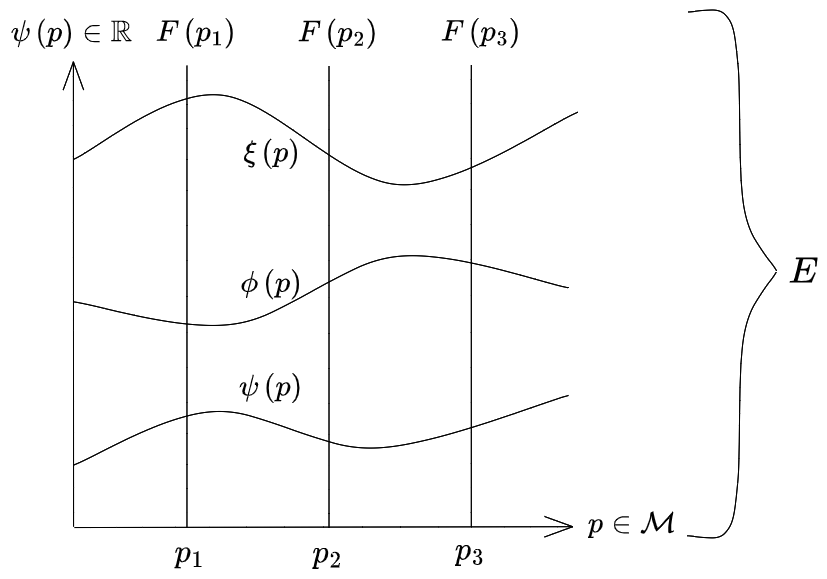
\includegraphics[scale=0.3]{bundle}
\caption{A bundle $E \overset{\pi}{\to} \mathcal{M}$. Note that $\psi \sim \phi \sim \xi$.}
\end{figure}
\end{frame}

\section{Topological Notions}

\subsubsection{Topological Bundles}
\begin{frame}{Topological Bundles}
\begin{itemize}
\item In topology, a bundle is constructed by considering a total [topological] space $\left( E, \mathcal{O}_{E} \right)$, a base space $\left( B, \mathcal{O}_{B} \right)$ and a continuous surjection $\pi : E \to B$.

$\left( E, \pi, B \right)$ or $E \overset{\pi}{\to} B$ is then said to be a [topological] bundle.

\item The fibre at a point $p \in B$ is defined as,

\begin{align*}
F \left( p \right) & : = \text{preim}_{\pi} \left( \left\{ p \right\} \right) \\
& : = \left\{ x \in B : \pi \left( x \right) = \left\{ p \right\} \right\}
\end{align*}

\item A fibre bundle $\left( E, B, \pi, F \right)$ or $F \to E \overset{\pi}{\to} B$ is a structure where $E \overset{\pi}{\to} B$ is a bundle and every fibre is homeomorphic to a manifold $F$, called the typical fibre of the fibre bundle,

$$\forall x \in E : \text{preim}_{\pi} \left( \left\{ x \right\} \right) \cong_{\text{top}} F$$
\end{itemize}
\end{frame}

\subsubsection{Total Space}
\begin{frame}{Total Space}
\begin{itemize}
\item In the field-theoretic situation we considered earlier, the total space associated with a rank $\left( p, q \right)$ field on a spacetime $\mathcal{M}$ is typically homeomorphic to a manifold of dimension $\dim \left( \mathcal{M} \right) + p + q$.
\item We will consider Newtonian gravitation and classical electrodynamics on 3-dimensional Euclidean, and 4-dimensional Minkowski space, respectively. 
\item In the case of the Newtonian gravitational field $\phi$, the total space is $\mathbb{R}^3 \times \mathbb{R}$ and this can be equipped with the Euclidean topology $\mathcal{O}_{\mathbb{R}^4}$.
\item For the electromagnetic 4-potential $A$, the total space is $\mathbb{R}^4 \times \mathbb{R}^4$. This is Lorentzian, but we can make it Euclidean after a Wick rotation. In other words, the total space is isomorphic to $\mathbb{R}^8$, which can then be equipped with the Euclidean topology $\mathcal{O}_{\mathbb{R}^8}$.
\end{itemize}
\end{frame}

\subsubsection{Product Bundle Structure}
\begin{frame}{Product Bundle Structure}
\begin{itemize}
\item With the above constructions, we find that the canonical projection $E \to \mathcal{M}$ we defined earlier is indeed continuous and surjective, for both the gravitational potential and electromagnetic 4-potential fields.

\item Therefore, $\left( \mathbb{R}^3 \times \mathbb{R}, \pi_{\mathbb{R}^3}, \mathbb{R} \right)$ is a bundle, known as a product bundle. The same goes for $\left( \mathbb{R}^4 \times \mathbb{R}^4, \pi_{\mathbb{R}^4}, \mathbb{R}^4 \right)$ in the case of the electromagnetic field in flat spacetime.

\item Furthermore, in each case, the fibres are isomorphic to $\mathbb{R}$ and $\mathbb{R}^4$, respectively. This means that the product bundles above are also fibre bundles.
\end{itemize}    
\end{frame}

\subsubsection{Sections}
\begin{frame}{Sections}
\begin{definition}[Section]
A [cross-]section $s$ of a bundle $E \overset{\pi}{\to} B$ is as a continuous inverse of $\pi$,

$$\pi \circ s = \text{id}_{B}$$
\end{definition}

Sections can be visualized in the following manner:

\begin{figure}[H]
\centering
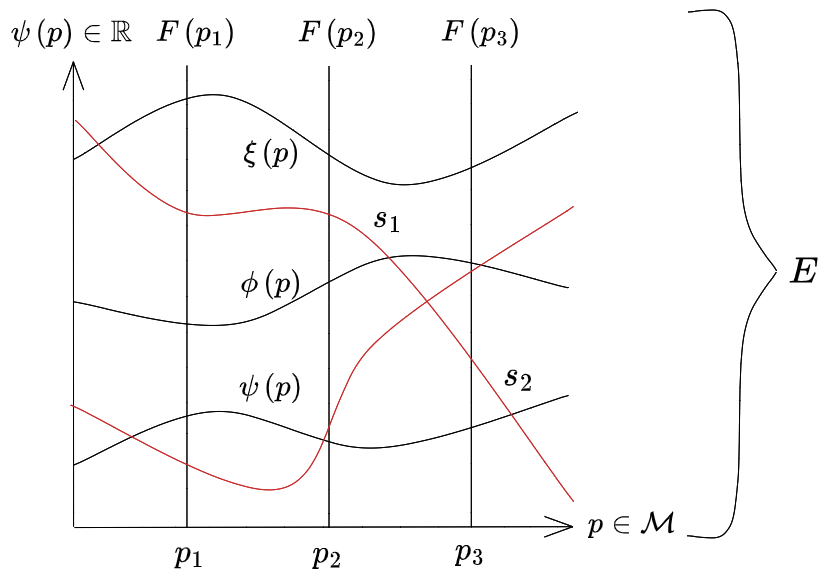
\includegraphics[scale=0.2]{section}
\caption{$s_1$ and $s_2$ are sections of the bundle $E \overset{\pi}{\to} B$.}
\end{figure}
\end{frame}

\begin{frame}{}
\begin{itemize}
\item In the modern, geometric construction of classical field theory, classical fields are defined as sections of fibre bundles.
\item The typical fibres of these fibre bundles are usually Lie groups (which are manifolds, as required).
\end{itemize}
\end{frame}

\begin{frame}{References}
\begin{enumerate}
\item \emph{The Geometrical Anatomy of Theoretical Physics}, Frederic P. Schuller
\item \emph{From Special Relativity to Feynman Diagrams}, Riccardo D'Auria, Mario Trigiante
\item Wikipedia
\end{enumerate}
\end{frame}

%\begin{frame}[allowframebreaks]
%\frametitle{References}
%\printbibliography
%\end{frame}
\end{document}